\chapter{Parallel Implementation}
\label{cha:parallel_implementation}

Based on the previous two chapters describing the serial Fortran implementation and GPU programming we will now look at the algorithm in more detail and show, how it was adapted to take advantage of multi-core architectures. The main focus of this thesis is the implementation of the simulation on a modern massively parallel NVIDIA GPUs using CUDA. In order to gain a better understanding of the achievable performance improvements we additionally back-ported the finished GPU code of the algorithm to multi-core CPUs using the OpenMP framework.

We will begin by introducing the software tools and libraries utilized. Afterwards, we will explain the practical implementation of the algorithm in CUDA. This is followed by the discussion of several potential optimization approaches to further improve the performance of the simulation. The chapter ends with a brief explanation of OpenMP and how the code was parallelized on the CPU.

\section{Development environment}

The rigid fiber simulation developed as part of this thesis is only loosely based on the original serial Fortran implementation. This was done to ensure a clean starting point and avoid difficulties in adapting the existing code for parallel execution, as it was never intended to be run across multiple cores. This also provided the opportunity to learn from the shortcomings of the old code to not only parallelize it but also improve the efficiency in general.

The development was done exclusively on a Linux workstation running Ubuntu as this will also be the exact same runtime environment used in the later experimental usage of the resulting application. The build system for compiling and linking the final application was CMake. It was chosen because it is a widely used open-source and cross-platform build system, which allows for easy integration of the various required libraries in a well documented and straightforward manner.

Under the hood the build system uses NVIDIA's CUDA platform tools to compile the code. For this NVIDIA includes \emph{nvcc}, an LLVM-based CUDA compiler capable of compiling C/C++ code together with the CUDA specific extensions.

In order to facilitate easier usage of the application both during development and later real-world usage a Python wrapper script is also available. The script completely automates the building process and dynamically customizes the application code to support three different modes of operation. The first is a simple \emph{run} mode which takes the supplied parameters and executes the simulation. The second mode is \emph{validate}, it allows for a fully automated way to test and validate different algorithm variations against a known correct simulation run. This includes automatically computing the error as well as the error location in the matrix allowing for easier debugging of changes. The last mode is \emph{benchmark} which runs the supplied parameters through a series of iterations collecting and aggregating timings for each simulation step as well as the total time.

\section{Linear Solvers}
In addition to the CUDA platform, the application also requires support libraries for the different linear solvers. It is very important to weigh all the options when choosing a particular linear solver algorithm or library, because solving the system can be one of the most time consuming steps. So the overall simulation time relies heavily on the ability to solve large and dense systems as fast as possible. The two main libraries are \emph{MAGMA} for the direct solver and \emph{ViennaCL} for the iterative solvers. Both will be introduced briefly now.

\paragraph{MAGMA / CuBLAS / OpenBLAS}
The MAGMA project contributes the implementation for the direct solver used in this thesis. This dense linear algebra library provides features similar to standard LAPACK functions but for multicore architectures. It also has features to support hybrid algorithms to run code across multiple GPUs or CPUs at the same time, however, these features were not explored in this thesis. Instead the focus was on a high performance single GPU implementation of a direct linear system solver.

MAGMA provides access to various high-level algebra routines, but the underlying math functions utilize the platform specific implementations of the BLAS levels. For CUDA this is implemented directly by NVIDIA in the form of the CuBLAS libraries. Additionally, MAGMA tries to further improve their performance by combining GPU with CPU based algorithms. Thus a CPU based BLAS implementation is also needed. For this the OpenBLAS library was chosen which is the most up-to-date and high performance library available outside the very expensive Intel MKL library. OpenBLAS takes full advantage of multicore systems and is also used for the comparison of Fortran CPU implementation against the CUDA GPU implementation.

\paragraph{ViennaCL}
ViennaCL is an open-source linear algebra library developed at the University of Vienna. The library provides an abstraction layer across many different parallelization methods in order to facilitate consistent and easy to use support for BLAS level 1-3 and iterative solvers. This unique feature allows the developer to easily switch between different backends for parallelization. Currently, the library supports OpenMP, OpenCL and most importantly for this thesis - CUDA.

ViennaCL's focus is on solving sparse matrices with the implemented iterative solvers. However, it also has basic support for solving dense matrices using a variety of different iterative solvers. As the rigid fiber simulation exclusively relies on dense matrices this makes it an ideal candidate for benchmarking. For this thesis the BiCGStab as well as the GMRES iterative solvers were used and tested.

\section{Kernels}
\label{sec:kernels}

The overall parallel algorithm is very similar to the serial version, however, each simulation step is separated into different kernels. Each kernel is invoked in a serial manner, this means CUDA guarantees that all data modified in a kernel is available before the next kernel is executed. These kernels are then distributed across the GPU. All calculations are done using single precision floating point numbers, as NVIDIA limits high performance double precision computation to their server class GPUs. The CUDA pseudocode for the algorithm is illustrated in Listing~\ref{lst:pseudo_parallel_algorithm}. It begins by parsing the simulation parameters and the initial fiber configuration. After that, the required memory is allocated on the GPU. Finally a simple loop executes all time steps and the four main algorithm sub steps — 1. \emph{Assemble System}, 2. \emph{Solve System}, 3. \emph{Update Velocities} and 4. \emph{Update Fibers} — are run on the GPU.

\begin{listing}[!htbp]
  \centering
  \begin{minted}[mathescape,
    linenos,
    numbersep=5pt,
    fontsize=\footnotesize,
    frame=lines,
    framesep=2mm]{c}
    int main()
    {
    // Parsing algorithm parameters and initial fiber positions
    readParameters();
    readFiberConfiguration();
    allocateGPUMemory();
    ...

    for (int step = 0; step < max_timestep; step++)
    {
    AssembleSystem<<<numBlocks, threadsPerBlock>>>(...);
    SolveSystem<<<numBlocks, threadsPerBlock>>>(...);
    UpdateVelocities<<<numBlocks, threadsPerBlock>>>(...);
    UpdateFibers<<<numBlocks, threadsPerBlock>>>(...);
    }
    ...
    }
  \end{minted}
  \caption{Pseudocode for parallel algorithm on the host.}
  \label{lst:pseudo_parallel_algorithm}
\end{listing}

The application requires two general configuration files as an input. The first file is referred to as the parameters file which contains the different configuration variables and constants used throughout the algorithm. These include, for example the number and size of the time steps as well as the number of force expansion terms and quadrature points. Additionally, this file is also used to configure the iterative solvers like specifying the number of restarts for GMRES or the solution tolerance for BiCGStab and GMRES.

Each of the parallelized sub steps are now discussed in more detail. The purpose of each kernel as well as the required input and outputs.

\paragraph{Assemble System}

\begin{listing}[!htbp]
  \centering
  \begin{minted}[mathescape,
    linenos,
    numbersep=5pt,
    fontsize=\footnotesize,
    frame=lines,
    framesep=2mm]{c}
    __global__ void AssembleSystem1D(
    in float *positions,
    in float *orientations,
    out float *a_matrix,
    out float *b_vector)
    {
    const int i = blockIdx.x * blockDim.x + threadIdx.x;

    if (i >= NUMBER_OF_FIBERS) return;

    for (int j = 0; j < NUMBER_OF_FIBERS ++j)
    {
    for (int force_index_j = 0;
    force_index_j < NUMBER_OF_TERMS_IN_FORCE_EXPANSION;
    ++force_index_j)
    {
    computeInnerIntegral(...);

    for (int force_index_i = 0;
    force_index_i < NUMBER_OF_TERMS_IN_FORCE_EXPANSION;
    ++force_index_i)
    {
    // Only 1D thread block
    // Each thread updates unique memory locations, thus
    // no need for atomics
    setMatrix(...)
    setVector(...)
    }
    }
    }
    }
  \end{minted}
  \caption{Pseudocode for the assemble system step with a 1D thread block.}
  \label{lst:pseudo_assemble_system}
\end{listing}

The \emph{Assemble System} kernel is the most important step of the algorithm, as it is the most time consuming step. This was already discussed in section~\ref{sec:algorithm_summary} and we will also be shown during benchmarking in Chapter~\ref{cha:benchmarks}. The goal of this step is to build the matrix and vector in memory for the linear system of equations. As an example Listing~\ref{lst:pseudo_assemble_system} shows the pseudocode for the one-dimensional implementation of the \emph{Assemble System} step. This means the code is parallelized for each fiber and each thread calculates the contributions to this fiber from all other fibers. Looking at the matrix in equation~\eqref{eq:matrix_structure} each thread is thus responsible for $3*N$ rows of the matrix, where $N$ is the total number of terms in the force expansion. Alongside the one-dimensional implementation other options exist. They will be discussed in the optimization section~\ref{sec:parallel_optimizations}.

The kernel requires two inputs, the current position of each fiber and its orientation. Using these combined with the equations outlined in Chapter~\ref{cha:theoretical_foundation} and Chapter~\ref{cha:serial_implementation} the matrix and vector elements are computed and used in the next step to solve the linear system they define.

\paragraph{Solve System}
As this thesis does not aim to implement generic linear solvers, this step is treated as a black box. During the previous \emph{Assemble System} kernel two arrays containing the matrix and right hand side of the linear system have been computed. These two arrays are now passed to the respective function of the library containing the linear solver. This is the MAGMA library in case of the direct solver and the ViennaCL library in case of the two tested iterative solvers BiCGStab and GMRES. Both libraries are able to directly use the already allocated memory regions and no additional allocations have to be performed. In order to conserve memory space the resulting solution vector is stored in the same memory location as the $b$-vector and is passed on to the subsequent steps.

\paragraph{Update Velocities}

\begin{listing}[!htbp]
  \centering
  \begin{minted}[mathescape,
    linenos,
    numbersep=5pt,
    fontsize=\footnotesize,
    frame=lines,
    framesep=2mm]{c}
    __global__ void UpdateVelocities2D(...)
    {
    const int i = blockIdx.x * blockDim.x + threadIdx.x;
    const int j = blockIdx.y * blockDim.y + threadIdx.y;

    if (i >= NUMBER_OF_FIBERS) return;
    if (j >= NUMBER_OF_FIBERS) return;
    if (i==j) return;

    for (int quadrature_index_i = 0;
    quadrature_index_i < TOTAL_NUMBER_OF_QUADRATURE_POINTS;
    ++quadrature_index_i)
    {
    for (int quadrature_index_j = 0;
    quadrature_index_j < TOTAL_NUMBER_OF_QUADRATURE_POINTS;
    ++quadrature_index_j)
    {
    force = computeForce(coefficients, ...)
    computeDeltaVelocities(force)
    }
    }

    // 2D thread block
    // Each thread responsible for an interaction pair, thus
    // result is written to the same memory location
    // Using atomics to avoid conflicts
    atomicAdd(&(translational_velocities[i].x),
    delta_translational_velocity.x);
    atomicAdd(&(translational_velocities[i].y),
    delta_translational_velocity.y);
    atomicAdd(&(translational_velocities[i].z),
    delta_translational_velocity.z);

    atomicAdd(&(rotational_velocities[i].x),
    delta_rotational_velocity.x);
    atomicAdd(&(rotational_velocities[i].y),
    delta_rotational_velocity.y);
    atomicAdd(&(rotational_velocities[i].z),
    delta_rotational_velocity.z);
    }
  \end{minted}
  \caption{Pseudocode for the updating velocities simulation step.}
  \label{lst:pseudo_update_velocities}
\end{listing}

After solving the linear system the solution coefficients are used to update the velocities of the fibers. The \emph{Update Velocities} kernel accumulates the exerted forces for all fibers and updates both the translational and the rotational velocities simultaneously. In this particular instance the 2D thread block version of the kernel is illustrated in Listing~\ref{lst:pseudo_update_velocities}. This means each individual kernel invocation is responsible for a single pair of fiber interactions. In case two different threads calculate the interactions for the same fiber, it might happen that they try to write their results to the same memory location. When this happens, it could to undefined behavior and incorrect results for the velocities. Fortunately CUDA provides a mechanism to circumvent this issue.

By using the so-called atomic functions CUDA streamlines and serializes the memory access. Thus the \emph{atomicAdd} function accumulates different velocity contributions to a fiber from all the other fibers. This ensures that each update to the memory location is handled in a serial manner, guaranteeing the correct value in memory. Of course this implies a potential performance degradation, however, newer GPUs with new CUDA versions have been very well optimized to only have a minimal impact. Benchmarking for the fibers simulation shows that using a 2D thread block and the associated performance increases far outweigh the potential performance hit of using atomics.

\paragraph{Update Fibers}

\begin{listing}[!htbp]
  \centering
  \begin{minted}[mathescape,
    linenos,
    numbersep=5pt,
    fontsize=\footnotesize,
    frame=lines,
    framesep=2mm]{c}
    __global__ void UpdateFibers()
    {
    int i = blockIdx.x * blockDim.x + threadIdx.x;

    if (i >= NUMBER_OF_FIBERS) return;

    next_positions[i] = 4/3 * current_positions[i]
    - 1/3 * previous_positions[i]
    + 2/3 * TIMESTEP
    * (2 * current_translational_velocities[i]
    - previous_translational_velocities[i]))

    next_orientations[i] = 4/3 * current_orientations[i]
    - 1/3 * previous_orientations[i]
    + 2/3 * TIMESTEP
    * (2 * current_rotational_velocities[i]
    - current_rotational_velocities[i]))

    normalize(next_orientations)
    }
  \end{minted}
  \caption{Pseudocode for the updating fibers simulation step.}
  \label{lst:pseudo_update_fibers}
\end{listing}

The final simulation step takes care of advancing the position and orientation of the fibers in time. The pseudocode in Listing~\ref{lst:pseudo_update_fibers} implements the second-order multi-step method introduced in section~\ref{sec:serial_update_fibers}. As it will be shown later during benchmarking in Chapter~\ref{cha:benchmarks}, the required time for this kernel is minuscule compared to the other steps. The kernel only scales linearly and in addition has a perfectly aligned memory access resulting in close to optimal usage of the GPU hardware.

\section{Optimizations}
\label{sec:parallel_optimizations}

During the development of the parallel GPU simulation great care was taken to continuously optimize the code both on an algorithmic level as well as on an implementation level. Numerous small code-level optimizations have been performed based on the original serial code like precomputing as much data as possible, avoiding variable allocations or unnecessary copy operations in performance critical sections of the code.

Additionally, more advanced optimization were made like rearranging calculations inside loops to avoid executing redundant calculations and consolidating multiple loops into one. Finally, techniques such as loop unrolling and faster math functions where also tested and included.

Throughout the optimization phase the benchmark suite was run after each step. This ensures that optimizations were only included if they had a measurable impact on the overall performance of the simulation. Moreover, with this approach potential performance regressions could be identified early and be avoided.

Many optimizations performed during this process are applicable to both the CPU and GPU, since they showed performance improvements for both. However, some optimizations and algorithm variations are uniquely suited to the GPU hardware. For this thesis we will look into three different optimizations on the GPU in more detail. The performance results for each will then later be discussed in Chapter~\ref{cha:benchmarks}.

\subsection{Numeric vs. Analytic Integration}
\label{subsec:numeric_analytic}
The first optimization was already part of the original serial implementation as described in section~\ref{subsec:inner_integral}. In the original paper \cite{Tornberg2006} the authors observed that the analytical integration of the inner integral yielded a performance increase compared to the purely numerical integration. Generally an analytical integration should not only be preferred because of being faster but more importantly also because of being more accurate. However, for numerical precision reasons the actual implementation of the analytical integration can't achieve this theoretical level of accuracy. Especially for configurations with fibers that are very far apart the recursive implementation suffers from round-off errors and numerical instabilities. The steps taken to minimize these instabilities potentially affect the performance.

Based on these considerations and the fact that the computation of the integrals is a very performance critical part of the implementation, exploring the performance implications of both approaches on the GPU is of great interest. In contrast to the serial CPU implementation of the original paper, our implementation on the GPU is actually faster when solving both integrals numerically. We will discuss the reason and consequences of this in more detail in section~\ref{subsec:bench_numeric_vs_analytic}.

\subsection{Shared Memory}
\label{subsec:shared_memory}

As described in section~\ref{sec:CUDA} CUDA code is subject to a highly specialized memory hierarchy. Whereas traditional CPUs only have small caches and a large main memory pool, CUDA introduces the concept of a shared local memory space. The access time to this local memory is orders of magnitudes faster compared to accessing the global GPU memory. Additionally, local memory can be shared among the threads running on Streaming Multiprocessor and potentially save time by avoiding to constantly access the slow global memory.

In order to test this, shared memory was implemented and tested with the \emph{Assemble System} step, the most performance critical kernel. To understand the idea, imagine the 2D thread block implementation of the kernel. Each thread block is responsible for many pairs of fiber interactions, e.g. fibers $[1,\dots,8]$ each interacting with fibers $[9,\dots,16]$. In total, these are $8 \times 8 = 64$ interactions. Each kernel invocation is responsible for one pair and has to load the position and orientation for the two interacting fibers. However, on closer inspection it is obvious that one does not need to load each fiber every time. As soon as fiber $1$ has been loaded into shared memory it can be reused for all the interactions with fibers $9$ through $16$ avoiding the unnecessary and slow access to global memory.

How this affects performance is not always easy to tell, as various factors can influence the result. One factor, for example might be that the loaded data is small enough and repeated access to global memory can be automatically avoided by taking advantage of other memory caches. Another factor is performance characteristic of the kernel. Optimizing for shared memory usage only makes sense if the kernel is memory bound, meaning that most of the execution time is spent waiting for data. If on the other hand the kernel is compute bound the GPU is able use time effectively by performing pending computations while waiting for memory access. In this case forcing threads in a block to wait for shared data can actually decrease the overall performance of the kernel.

However, in general efficient exploitation of shared memory can be a huge advantage for parallel GPU implementations. This is especially true when comparing the performance to CPUs, as they don't have an equivalent fast and comparatively large memory space. Unfortunately, during our testing in section~\ref{subsec:bench_shared_memory} the effect for the GPU simulation of rigid fibers proved to be rather limited.

\subsection{Thread Block Dimension}
\label{subsec:bench_thread_block}

There are many different factors that determine the performance of a particular GPU algorithm. This is especially true with regard to optimally taking advantage of the specific underlying GPU architecture, which change even between different models of graphics cards. How to best utilize the hardware depends on specific memory access patterns, avoiding too much register usage and choosing optimal settings for the thread block size. Each graphics cards can have a different number of streaming multiprocessors with only limited resources and taking advantage of this can result in performance increases.

For this thesis we looked at the Thread Block dimension in particular and how choosing a different approach of parallelizing affects the performance. Doing so, the focus was on the \emph{Assemble System} step, which is the most performance critical step. However, the results were then also transferred to the \emph{Update Velocities} step.

The most straight forward approach is to simply parallelize the algorithm with regard to a single fiber. This means each kernel invocation is responsible for calculating all the interactions for this fibers with all other fibers. In this way a single kernel is responsible for multiple rows of the resulting linear system matrix. Additionally, this approach does not have any memory access conflict as each kernel only writes to the memory location belonging to its unique fiber. The potential disadvantage for a one-dimensional thread block, however, is that the resulting code can be more resource intensive for each single kernel and potentially hinder the performance on each multiprocessor.

For a two-dimensional thread block each kernel invocation is responsible for a pair of interacting fibers. While this decreases the necessary resources, it also requires atomics which can potentially slow down the execution. Three-dimensional thread blocks are the maximum allowed dimensions for a CUDA thread block. They are a further extension of the two-dimensional thread block, as now each kernel invocation is not responsible for the complete interaction but only the interaction resulting from a specific point of the force expansion. This results in even more potential memory conflicts and also increases the total number of thread blocks which have to be distributed.

The kernel invocations for the one-dimensional and two-dimensional thread block approach are visualized using the matrix structure in equation~\eqref{eq:matrix_structure}, as shown in Figure~\ref{fig:thread_block}. In the one-dimensional case each invocation is responsible for all sub matrices $\bar{A}_{ml}$ describing the contribution from the force coefficients on fiber $l$ on to the force coefficients for fiber $m$. Thus in total this results in $M$ kernel invocations, one for each fiber. For the two-dimensional case each invocation is only responsible for a single sub matrix. Here the total number of invocations is $M \times M$. The three-dimensional case then divides the calculation for the sub matrix further, one additional invocation per force index for a total of $M \times M \times N$ invocations.

\begin{figure}[!htbp]
  \centering
  \begin{subfigure}[h]{0.33\textwidth}
    \centering
    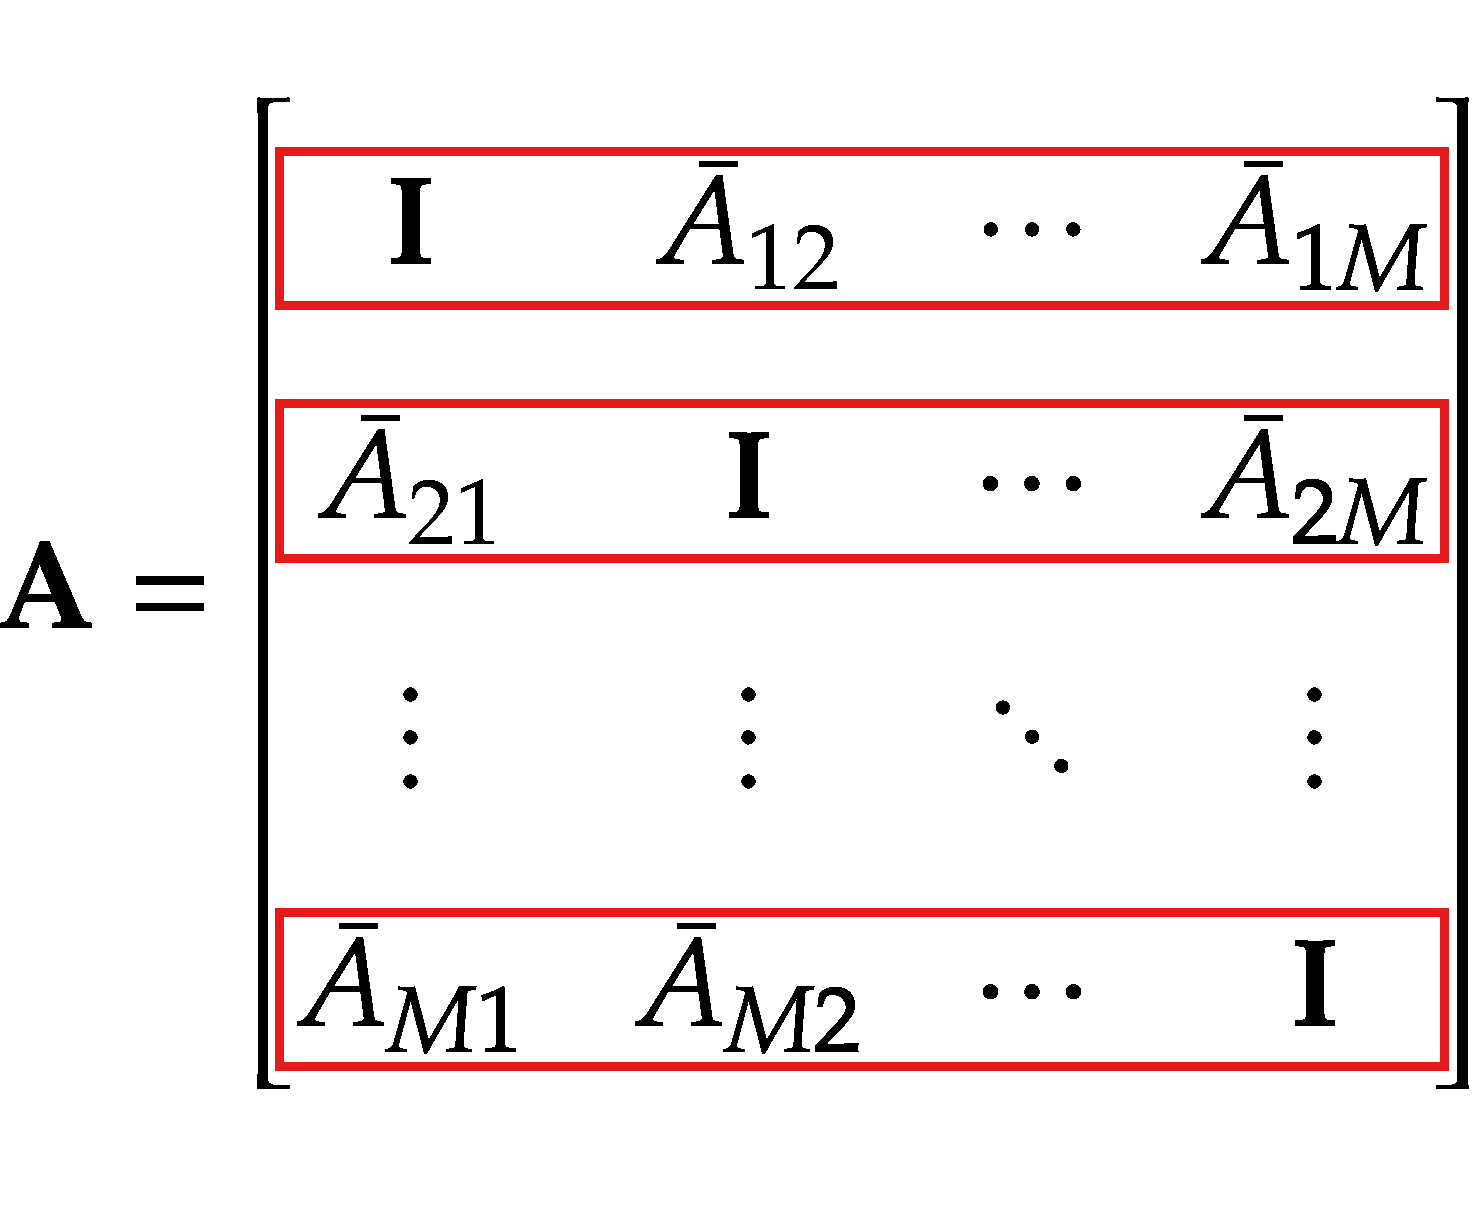
\includegraphics[width=\textwidth]{img/thread_block1D.pdf}
    \caption{1D}\label{fig:thread_block_1D}
  \end{subfigure}
  \begin{subfigure}[h]{0.33\textwidth}
    \centering
    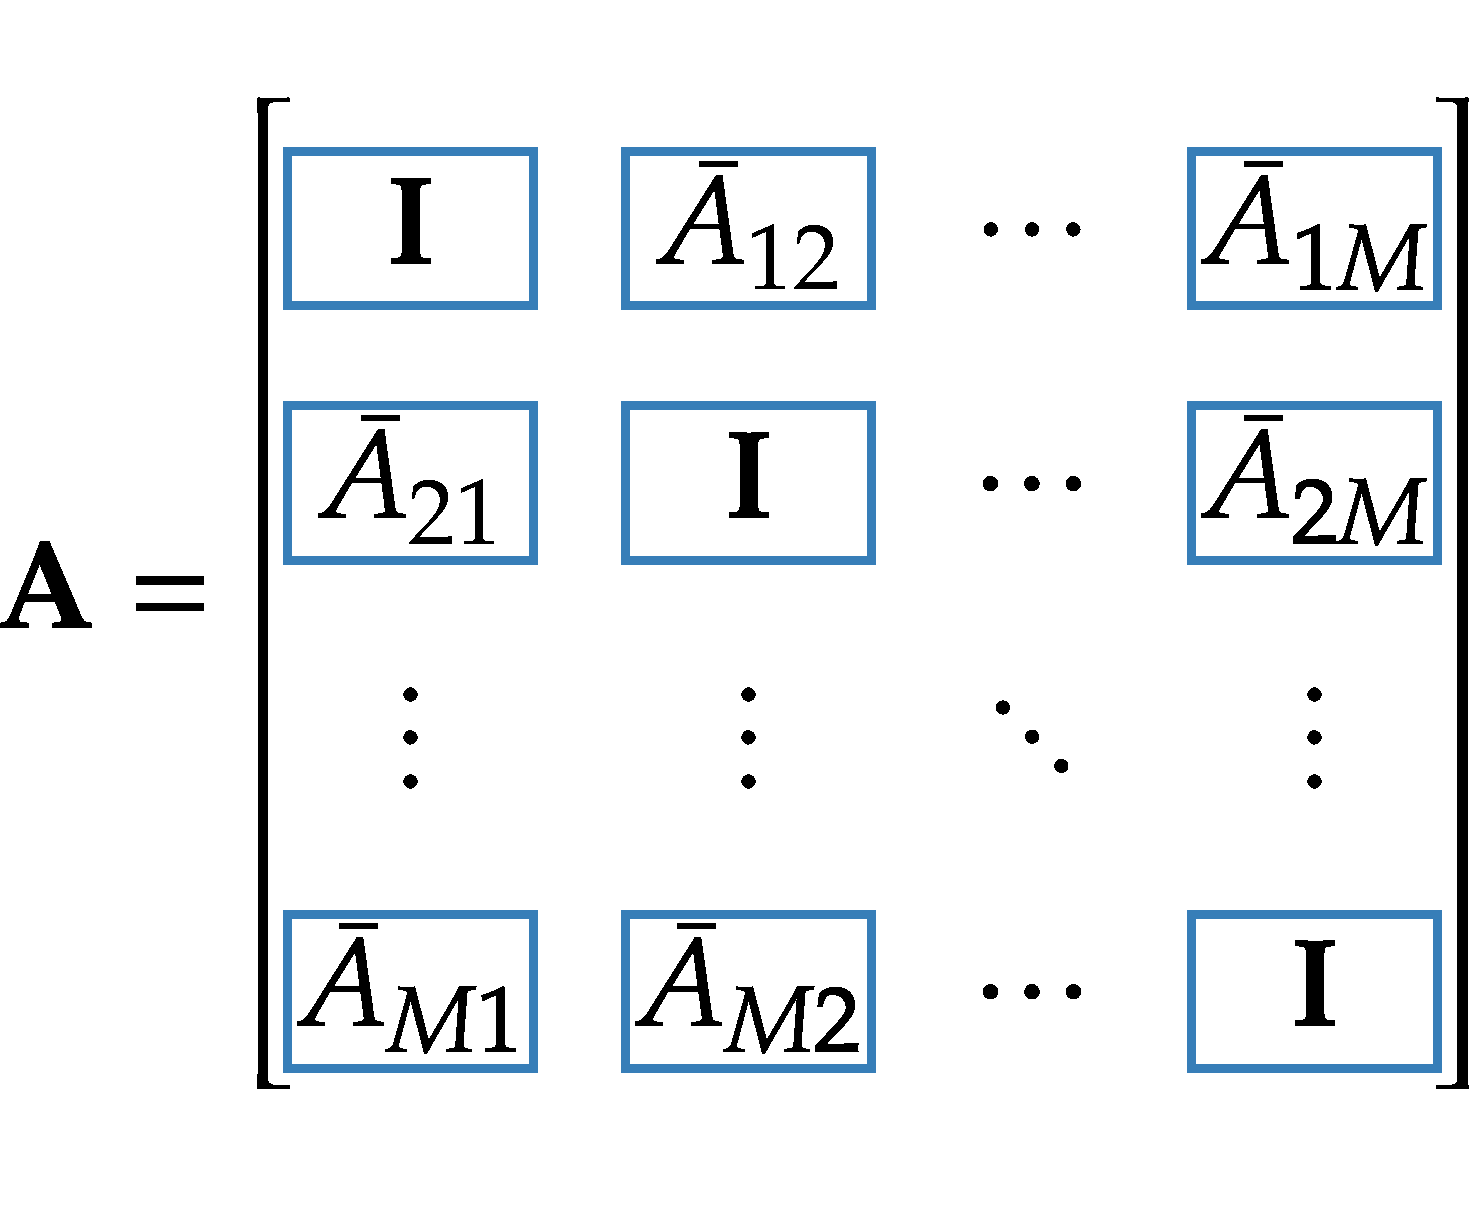
\includegraphics[width=\textwidth]{img/thread_block2D.pdf}
    \caption{2D}\label{fig:thread_block_2D}
  \end{subfigure}
  \caption{Illustration of 1D and 2D thread block dimension using simulation system matrix.}
  \label{fig:thread_block}
\end{figure}

It is not clear, how exactly the performance is affected by each decision for the thread block dimension. Only trial-and-error benchmarking combined with metrics from CUDA can find the optimal setting for the specific algorithm. We will later show in section~\ref{subsec:bench_thread_block}, that for our GPU implementation the two-dimensional approach is the most efficient one.

\section{OpenMP}

The goal of this thesis is to implement a high performance rigid fiber simulation on the GPU using CUDA. In order to better understand to what degree this goal was achieved, it is crucial to have a comparison. The original serial implementation is not an ideal candidate as it does differ in a number of ways. First of all, it is purely serial and doesn't take advantage of todays multicore CPUs. Furthermore, it was implemented in double precision and because of arbitrary restrictions NVIDIA places on its consumer GPUs, they are only suited for single precision. That is why the CUDA implementation is strictly single precision. Finally, the primary focus of the original Fortran implementation was a correctly implemented algorithm and not performance.

For these reasons and in order to have a fairer comparison of the performance differences between the GPU and CPU implementation, a completely new and rewritten parallel CPU simulation was also implemented. For the parallelization on the CPU the OpenMP library was chosen.

After having implemented a parallel algorithm for the GPU, the conversion to the OpenMP-based CPU implementation was relatively straightforward. All optimizations done for the GPU implementation were also applied to the new CPU code when applicable. In order to parallelize the BLAS functions required for the linear solver the already included OpenBLAS library was chosen. OpenBLAS is an open-source and highly optimized library and automatically parallelizes BLAS functions using pthreads across all available CPU cores. In contrast to the GPU implementation, the OpenMP version is only parallelized in one-dimension. This means that each core calculates the interactions for one fiber with all other fibers or put differently all matrix rows belong to one fiber. As the underlying number of independent threads is much lower on CPUs, different parallelization dimensions didn't have an impact during testing.

The end results of the practical implementation for this thesis is a highly optimized CUDA implementation for NVIDIA GPUs and additionally a parallelized and optimized Fortran OpenMP implementation for CPUs. The next chapter will now look at a number of performance metrics and compare them between the GPU and CPU.
